%%%%%%%%%%%%%%%%%%%%%%%%%%%%%%%%%%%%%%%%%
% Diaz Essay
% LaTeX Template
% Version 2.0 (13/1/19)
%
% This template originates from:
% http://www.LaTeXTemplates.com
%
% Authors:
% Vel (vel@LaTeXTemplates.com)
% Nicolas Diaz (nsdiaz@uc.cl)
%
% License:
% CC BY-NC-SA 3.0 (http://creativecommons.org/licenses/by-nc-sa/3.0/)
%
%%%%%%%%%%%%%%%%%%%%%%%%%%%%%%%%%%%%%%%%%

%----------------------------------------------------------------------------------------
%	PACKAGES AND OTHER DOCUMENT CONFIGURATIONS
%----------------------------------------------------------------------------------------

\documentclass[12pt]{diazessay} % Font size (can be 10pt, 11pt or 12pt)
\usepackage{mathptmx}
\usepackage{setspace}
\usepackage{amsmath}
% for author-year citation style
\usepackage[round]{natbib}
\usepackage{lscape}
\usepackage{graphicx}
\usepackage{scalerel}
\usepackage[export]{adjustbox}
\usepackage{siunitx}
\usepackage{subfig}

\graphicspath{ {./pics} }
\bibliographystyle{plainnat}
%----------------------------------------------------------------------------------------
%	TITLE SECTION
%----------------------------------------------------------------------------------------

\title{\textbf{A Hybrid Approach to Insincerity Detection}} % Title and subtitle

\author{\textbf{Mengxuan Lyu, Jinyue Feng} \\ \textit{University of Toronto}} % Author and institution

\date{\today} % Date, use \date{} for no date

%----------------------------------------------------------------------------------------

\begin{document}

\maketitle % Print the title section

%----------------------------------------------------------------------------------------
%	ABSTRACT AND KEYWORDS
%----------------------------------------------------------------------------------------

%\renewcommand{\abstractname}{Summary} % Uncomment to change the name of the abstract to something else

% \begin{abstract}
% Morbi tempor congue porta. Proin semper, leo vitae faucibus dictum, metus mauris lacinia lorem, ac congue leo felis eu turpis. Sed nec nunc pellentesque, gravida eros at, porttitor ipsum. Praesent consequat urna a lacus lobortis ultrices eget ac metus. In tempus hendrerit rhoncus. Mauris dignissim turpis id sollicitudin lacinia. Praesent libero tellus, fringilla nec ullamcorper at, ultrices id nulla. Phasellus placerat a tellus a malesuada.
% \end{abstract}

% \hspace*{3.6mm}\textit{Keywords:} lorem, ipsum, dolor, sit amet, lectus % Keywords

% \vspace{30pt} % Vertical whitespace between the abstract and first section

%----------------------------------------------------------------------------------------
%	ESSAY BODY
%----------------------------------------------------------------------------------------
\doublespacing % double space

\section{Introduction}

Despite Quora's policy of \textit{``Be Nice, Be Respectful''}, misleading or discriminative questions of various types still exist. In this project, we will primarily focus on questions with non-neutral tone, rhetorical questions, discriminative questions and questions that use sexual content as shock value. After reviewing sentiment analysis studies, we have found that sarcasm detection is an extensively studied topic in this field. However, there are few studies on the classification of insincere or toxic questions. A closer look at the linguistic backgrounds of sarcasm and insincere questions revealed that these two phenomena share many similarities, which we will discuss in details in section \ref{relations-to-sarcasm}. Therefore, we are motivated to transfer and extend sarcasm detection approaches to our project. 

The goals of this project are: 
\begin{enumerate}
\item to develop a model that detects insincere questions to improve the quality of online conversations; 
\item to experiment on how different word embeddings and classification techniques suit this particular problem; 
\item to present and visualize corpus statistical information with an emphasis on how these information affect the classification results; 
\item to explore the linguistic nature of insincere question expressions. 
\end{enumerate}

\subsection{Project Design}

\subsubsection{Text to Vector}

The first part of our project would be mapping text data into numerical space for the further downstream task of classification. Here we adopt three ways of converting.

\begin{itemize}
	\item Textual Space

This process involves preprocessing of texts including tokenization and PoS-tagging, feature extraction such as counting the number of adjectives, and application of machine learning algorithms such as Support Vector Machine (SVM) and Random Forests (RF) for classification. We will analyze features that have the highest impact on insincerity detection to reveal some statistical information concerning the expression profile of insincere questions. 

	\item Embedding Space

This approach requires the usage of libraries and the implementation of CNN-LSTM models using TensorFlow and PyTorch. We will have a closer examination of these techniques in the following literature review. In addition to the attempt of achieving satisfactory predictions, we will also visualize the relationships among word vectors to help explore the semantical information about insincere questions.

	\item Modularization and Integration

As we will discuss in the following sections, the combination of different modularized components in a classification process may yield better performance than any module alone. We intend to deploy innovative methods to merge the textual space and embedding space modules. 	
\end{itemize}

\subsubsection{Classification}

The second part would be implementing different models, including SVM, RF, and nerual networks as well, to perform classification over mapped data.


\section{Literature Review}

% In this literature review, we will first explain the relationship between sarcasm and insincere questions (section \ref{relations-to-sarcasm}). Then, we will present some feature extraction approaches that are particularly effective for sentiment analysis (section \ref{statistic-features}) and discuss word-embeddings (section \ref{word-embeddings}) which will form the primary basis of our neural networks. Finally, we will review neural networks models that have achieved state-of-art performance with a particular focus on sarcasm detection (section \ref{nn-models}). 

\subsection{Relations to Sarcasm} \label{relations-to-sarcasm}

As we have introduced before, a closely related topic to insincere question classification is sarcasm detection, which is a frequently researched area in sentiment analysis\citep{joshi2017}. Sarcastic messages and insincere questions share many similarities regarding their linguistic nature:

\begin{enumerate}
	\item \textbf{Sentiment Involvement.} Both sarcasm and rhetorical questions involve non-neutral sentiments under the disguise of a propositional or interrogative structure \citep{joshi2017, schmidt1977}. 
	\item \textbf{Presence of Indicative Words.} One type of insincere questions contain expressions of exclusive absoluteness, such as \textit{``if not"}; other rhetorical questions have non-deontic modal verbs and some other special particles that strongly indicate its persuasive, not interrogative, nature \citep{schmidt1977}. Similarly, sarcastic texts also involve indicative words, such as \textit{`like'} in \textit{``like you understand"} \citep{joshi2017}. 
	\item \textbf{Dropped Negation.} Many sarcastic sentences and rhetorical questions are meant to make a negative statement despite the absence of negation words  \citep{joshi2017, schmidt1977}. For instances, ``Having a cold is so fun" means ``Having a cold is not fun at all", and ``Can such a man be innocent?" means ``Such a man cannot be innocent."
	\item \textbf{Intended Victim.} Sarcastic comments can be used to mock a victim, and insincere questions can be discriminative or disrespectful against certain groups of people. The harmful components in both situations may be implicit or explicit. 
	\item \textbf{Violation of Truthfulness.} Sarcastic comments that violate truthfulness resemble insincere questions that are based on false premises. To understand such languages, the listener needs to know what is the true background information and how the truthfulness is violated\citep{joshi2017}. This can be a hard problem in natural language processing as it largely depends on knowledge about certain people or certain topics. However, it is also possible that the untruthful texts have syntactic or semantic characteristics that can become features of machine learning classification models.  
\end{enumerate}

Based on these linguistic characteristics, we hypothesize that methods that are successful in sarcasm detection will achieve satisfactory performance on insincerity detection. However, we also expect some challenges in transferring the classification approaches from sarcasm to insincerity detection problem. First and foremost, the five properites listed above do not directly serve as classification features for either problem. They merely prove the similarity between the two problem and form the basis of our hypothesis from a linguistic point of view. Second, sarcastic patterns that have been trained into accurate statistical classifiers for sarcasm detection do not directly apply to insincerity detection. For example, sarcastic messages often feature a conflict between opposing sentiments in the same sentence \citep{joshi2017}, which may not be a significant property of insincere questions. We would have to develop feature sets specifically designed for insincerity detection using both statistical feature selection methods and knowledge-based heuristics. Third, although deep learning-based approaches have achieved state-of-art performance and gained popularity in sarcasm detection \citep{joshi2017}, such studies typically focus more on the analysis of the models than the scientific nature of the phenomena. In other words, we observe a gap between the linguistic basis and the learning algorithms. The lack of explanations of why neural networks perform well on sarcasm detection increases the difficulty of transferring sarcasm detection models to our problem domain; however, we also consider this as an opportunity for us to contribute to the knowledge base of insincerity detection. 
% Features in textual space vs embedding space

\subsection{Statistics-Focused Features} \label{statistic-features}

Statistics-focused features in sentiment classification follows an established pattern where four types of features are frequently examined, namely term frequencies, parts of speech counts, the presence of opinion words, and negations\citep{medhat2014}. The most commonly used statistical feature selection methods include point-wise mutual information, Chi-square, and latent semantics indexing \citep{medhat2014}. Generally speaking, these methods measures the statistical relationship of word occurrence and class identification. These feature selection methods, combined with classifiers such as SVM, have been shown to be effective in certain sentiment analysis tasks \citep{medhat2014}.
 
In our study, we focus more on presenting corpus statistics and analyzing how such statistical information contribute to a neural-network based classification process. A particularly relevant study was conducted by \citet{barbosa2010}, where the authors presented a 2-step sentiment analysis method that only utilized an SVM model for the machine learning process, but its feature extraction methods allowed for robustness against noisy data. The researchers developed two feature sets designed to provide abstract representations of short texts: meta-features (including PoS tags and prior subjectivity and polarity) and syntactic features (namely frequencies of certain types of characters). The detection process was divided into two parts: subjectivity detection and polarity detection of the subjective texts. The experiment followed a traditional approach where the classifiers with highest information gain were created using Weka, and the learning process was completed using SVM algorithm\citep{barbosa2010}. Although this method no longer offers state-of-art performance, we still consider the feature selection methods valuable to our project. We intend to adapt the design in this study to obtain measurements of corpus statistics to feed as features into our neural network models. 
\subsection{Word Embeddings}

To embed our text data into vector space for the downstream tasks, we adopted word embeddings in addition to the statistics-focued features.

A study on word embedding-based features \citep{joshi2016} provides insights on how to combine word embeddings with feature selection. This work examined how features calculated from word embedding vectors could augment existing feature sets including n-grams, dictionary-based features, syntactical features and pattern-based features. More specifically, the researchers attempted to use word vector distances to detect context incongruity independent of sentiment changes. The results indicated that word embedding-based features enhanced performance \citep{joshi2016}. This method might be useful in our project for two reasons: 1) insincere questions may also contain context incongruity because of conflict between asking a question while making a statement; 2) questions that have discriminative or sexual language may be detected based on the semantic similarities to a set of sensitive keywords.  In this system, known sources of errors include multiple-sense-induced embedding issues, incapability to identify contextual information, and non-sarcastic metaphors\citep{joshi2016}. We expect the latter two points have lower impact on insincerity detection than sarcasm detection because contextual information and metaphors are less relevant to insincere questions than sarcastic messages. 



\subsection{Neural Networks Models} \label{nn-models}

% for citation, use \citep{} instead of \cite

Here we review several studies on sarcasm detection and sentiment analysis in the hope of transferring core concepts and methods to insincere question classification.

Compared to long texts that contain more contextual information, short texts sentiment analysis can be more challenging, and thus methods such as bag-of-words or n-grams are shown to be less effective \citep{barbosa2010, santos2014}. \citep{santos2014} proposed a deep CNN model that constructed word embeddings from character-level to sentence-level for sentiment analysis. The character-level embeddings captured morphological information and the word-level embeddings catch syntactical and semantical information \citep{santos2014}. Finally, the sentence-level representations were constructed upon concatenated character-level and word-level features. The word-level embeddings came from Word2Vec embeddings, and the character-level and sentence-level were obtained using convolutional layers that successively extracted local features in windows and maxed over these windows to get the global representation \citep{santos2014}. According to the results, the extracted features at sentence-level typically concentrated on several sentiment-bearing keywords. On the other hand, the contributions of character-level representations were not closely examined, so to what degree morphological and shape information benefited sentiment analysis was not clear. Our project will primarily focus on semantical and syntactical analysis, but we would also like to explore the advantages of character-level embeddings given enough time and resources. 

\citet{poria2017} presented a CNN architecture that contained in parallel a baseline 2-layer CNN model that directly process the text and three pre-trained models covering three types of clues (in particular, sentiments, emotions and personalities) that could be beneficial for sarcasm detection. These pre-trained models were trained on their benchmark datasets and then used for feature extraction on the sarcastic tweets datasets. Unlike the CNN model that specialized in obtaining textual information in depth \citep{santos2014}, the four-component CNN model proposed by \citet{poria2017} horizontally extracted information from different aspects. Although the baseline features (directly extracted from the word vectors) showed better predictions than all pre-trained models, the combination of the baseline and pre-trained models yielded the best performance \citep{poria2017}. To merge the outputs of the four parts, the researchers tested two methods: combining the outputs using SVM and appending extracted features from the pre-trained models into the baseline CNN hidden layers \citep{poria2017}.  The former method showed better results possibly because appending the extracted features into the baseline models compromised their meaningfulness.\\

Another sarcasm detection study \citep{ghosh2016} presented a CNN-LSTM-DNN neural networks model for semantic modeling, and this model architecture was particularly relevant to our project design. Consider that the information-bearing parts of text could exist anywhere, the choice of convolutional neural networks and recurrent neural networks was reasonable as both CNN and RNN were capable of capturing sequential temporal information. On top of the LSTM layers, the researchers added a fully-connected DNN layer to map the features into a more separable space. The combination of CNN, LSTM, and DNN showed more superior results than recursive SVM, two-layer CNN, and two-layer RNN models \citep{ghosh2016}. Consider the similarity between the tasks of this study and our project, we intend to construct our neural networks architecture following this CNN-LSTM pattern. 

\section{Experimental Setup}

\subsection{Overview}
\begin{figure}[ht]
	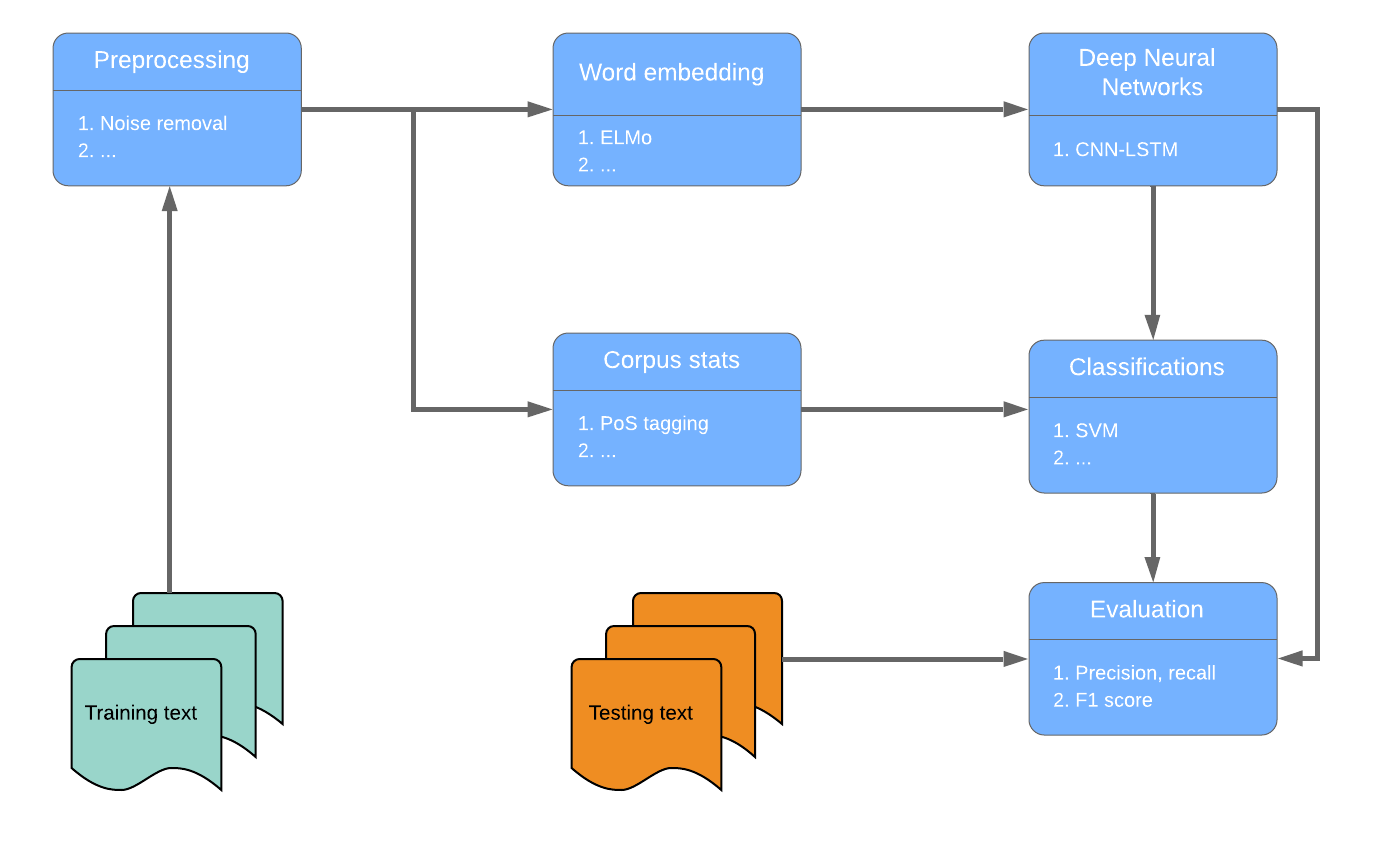
\includegraphics[width=0.6\textheight, center]{graphs/program_desi_flow.png}
	\caption{Program design}
	\label{figure:program_design}
\end{figure}
When designing this program, we implemented each part of the model into modules. As shown in Figure \ref{figure:program_design}, Quora question samples that are in textual form will be firstly embedded into numerical space with ELMo. Next, these embedded vectors will be fed into a CNN-LSTM network, which serves as our baseline model. Additionally, statistical features including PoS-tags, punctuation marks, named entities, and sentiment scores will be computed using existing libraries. The output of the baseline model and statistical features will then be merged using fully connected layers with dropout. The feature vector computed by the final hidden layer will then be fed to a softmax classifier. Evaluation metrics will be applied at the end of the experiments.

\subsection{Data Preparation} \label{data}
This project originates from a Kaggle challenge. Kaggle provides a dataset of $1,306,122$ questions with three fields \footnote{https://www.kaggle.com/c/quora-insincere-questions-classification/data}, namely \textit{qid} (a question id), \textit{question\_text} (the content of a question) and \textit{target} (where insincere questions are labeled as 1). 
% We will also be using word embeddings including \textit{Word2Vec, GloVe, ELMo} and \textit{BERT}. 

For the entire project, we rely on pandas library for data analysis because of its easiness to use and high performance. Our first step was to divide the dataset into a training set and a testing set in the ratio of 80:20. After a general analysis of the training set, we figured out that most of the questions were around 50 tokens in length, and there were only 22 sentences that were longer than 100 tokens. Thus we removed these 22 sentences to improve training efficiency. These process left us with \num[group-separator={,}]{1044839} training examples. 

We purposely did not treat our data with the commonly used stop-word removal step for our analysis except for unigram, because previous studies have shown that stop-word removal in twitter sentiment analysis tasks could hinder model performance given that the typical stop-word lists were not applicable to twitter corpus \citep{giachanou2016}. Similarly, stop words in short Quora questions may also serve as useful information for classification. 

Another pre-processing step we conducted was correcting one specific set of noisy data, namely questions involving mathematical formulas. The problem of wrongly labelled mathematical questions in this dataset is a known issue according to the Kaggle discussion forum. Since the presence of mathematical formulas could be a strong indicator of sincere questions, we want our model to accurately capture this information.

\subsection{Corpus Statistics} \label{corpus-stats}

For corpus statistics analysis, we used pandas for data handling, spaCy, textblob, and nltk for natural language processing, scipy for statistical testing, and matplotlib for plotting. 

In our current setup, we look into the statistical information in three major aspects: punctuation marks, parts-of-speech tags, and named entities. Although spaCy PoS-tagger includes PUNCT (punctuation) as one lexical category, we developed our own list of punctuation marks for finer-grained details. The PoS tags used followed the Universal Dependencies scheme \citep{pos-tag}, and the named entities list followed the categorization provided by spaCy Named Entity Recognition model trained on OntoNotes 5 corpus \citep{spacy-named-entity}. For each specific item in these three categories, we first compute the frequencies of an item in all sentences, and then conducted the Kolmogorov–Smirnov test (KS test) to compare their distributions in positive and negative samples. Since we used two-tail tests, the p-value threshold for significance is 0.01. All the tested features are listed in Table \ref{table:stats-features}. For all the significant features, we also generated boxplots, bar plots, and kernel density estimation graphs to visualize the distributions. 

Using KS test for discrete distributions is a compromised choice because the test is less powerful if the distributions are not continuous. The large sample size is also problematic as it reduces the power of significance testing. At this point, we use this test as a coarse filtering process. One benefit of this approach is that the conservative reduction of number of features allows us to conduct more comprehensive corpus statistics analysis. In later steps, we will incorporate more feature selection methods to further reduce feature dimensions if necessary. 

Another feature that we intend to add to our analysis is the sentiment measurements from textblob library. We believe that directly feeding sentiment information to our model would be beneficial because a non-neutral tone is one of the main indicators of insincere questions. 

\begin{table}[ht!]
\resizebox{\textwidth}{!}{%
\begin{tabular}{|l|l|l|l|ll}
\cline{1-4}
& punctuation marks & PoS tags & named entities &  &  \\ \cline{1-4}
\begin{tabular}[c]{@{}l@{}}Statistically \\ Significant \\ Features\end{tabular} & \begin{tabular}[c]{@{}l@{}}all punctuation marks \\- (from string.punctuations)\\ commas\\ periods\\ quotation marks\\ question marks\\ other punctuation marks\end{tabular} & \begin{tabular}[c]{@{}l@{}}ADJ: adjective\\ ADP:  adposition\\ ADV:  adverb\\ CCONJ:  coordinating conjunction\\ DET:  determiner\\ NOUN:  noun\\ NUM:  numeral\\ PART:  particle\\ PRON:  pronoun\\ PROPN:  proper noun\\ VERB:  verb\end{tabular} & \begin{tabular}[c]{@{}l@{}}PERSON\\-  People, including fictional. \\ NORP\\-  Nationalities or religious or political groups. \\ ORG\\-  Companies, agencies, institutions, etc. \\ GPE\\-  Countries, cities, states. \\ LOC\\-  Non-GPE locations, mountain ranges, bodies of water. \\ DATE\\-  Absolute or relative dates or periods. \\ CARDINAL\\-  Numerals that do not fall under another type.\end{tabular}                      &  &  \\ \cline{1-4}
others                                  & exclamation marks                     & \begin{tabular}[c]{@{}l@{}}AUX: auxiliary\\ INTJ: interjection\\ SCONJ: subordinating conjunction\\ SYM: symbol\\ X: other\end{tabular}          & \begin{tabular}[c]{@{}l@{}}FAC\\-  Buildings, airports, highways, bridges, etc.\\ PRODUCT\\-  Objects, vehicles, foods, etc. (Not services.)\\ EVENT\\-  Named hurricanes, battles, wars, sports events, etc.\\ TIME\\-  Times smaller than a day. \\ PERCENT\\-  Percentage, including "\%". \\ MONEY\\-  Monetary values, including unit. \\ QUANTITY\\-  Measurements, as of weight or distance. \\ WORK\_OF\_ART\\-  Titles of books, songs, etc. \\ LAW\\-  Named documents made into laws. \\ LANGUAGE\\-  Any named language.\\ ORDINAL\\-  "first", "second", etc.\end{tabular} &  &  \\ \cline{1-4}
\end{tabular}%
}
\caption{Features for KS tests}
 \label{table:stats-features}
\end{table}


To visualize extracted statistical features about punctuation, parts-of-speech tag, and named entities at corpus level, we created bar plots for the counts of the occurrences over the entire corpus. To visualize the distributions at sentence level, we used boxplots. For certain features of which the distributions are extremely skewed, our visualization methods may not provide the best representation. We have tried to use different types of plots to complement each other to partially solve this problem. For example, we created pie chart for punctuation marks to show the relative distribution in one sample population. Among the three aspects, the graphs showing the distributions of parts-of-speech tags are the most informative. As we are still refining these visualization techniques, here we only present some examples (Figure \ref{figure:pos_bar}, Figure \ref{figure:verb_box}, Figure \ref{figure:puncpie}) to show our progress. 

\begin{figure}[ht]
	\centering
	\subfloat[noun]{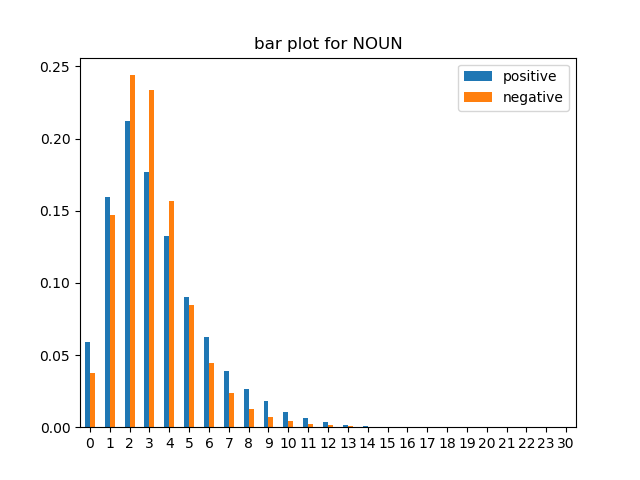
\includegraphics[width=0.5\textwidth]{graphs/noun_bar.png}}
	\subfloat[verb]{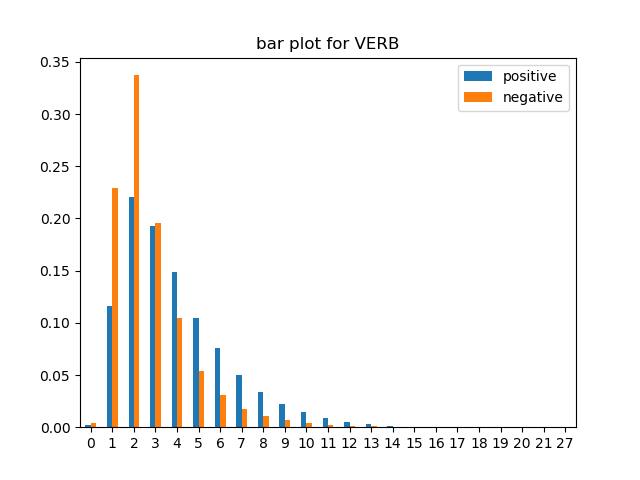
\includegraphics[width=0.5\textwidth]{graphs/verb_bar.png}}
	\caption{Bar plots of normalized counts of PoS tags in positive and negative samples}
	\medskip
	\small
	Positive sentences are labelled as insincere. The y-axis is the normalized counts and x-axis is the number of occurrences of a pos tag in a sentence. 
	\label{figure:pos_bar}
\end{figure}


\begin{figure}[ht] 
	\centering
	\subfloat[noun]{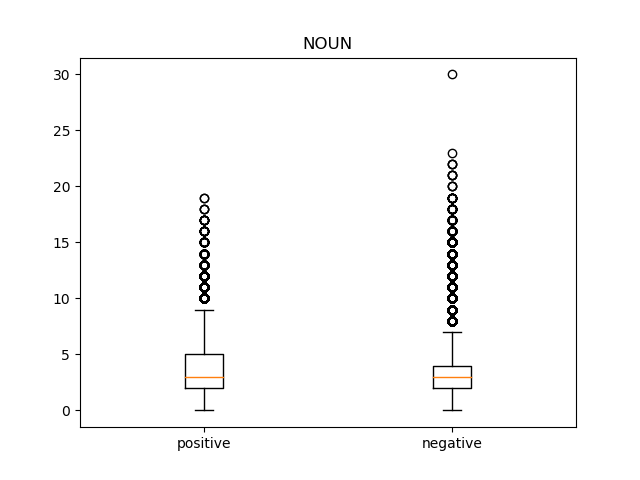
\includegraphics[width=0.5\textwidth]{graphs/noun_box.png}}
	\subfloat[verb]{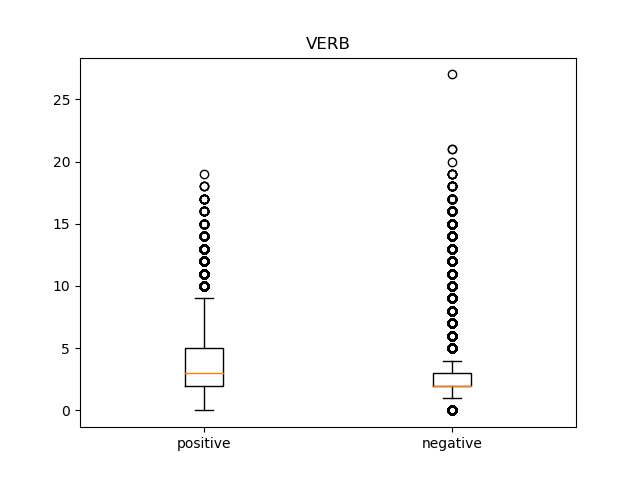
\includegraphics[width=0.5\textwidth]{graphs/verb_box.png}}
	\caption{Boxplot for the distribuition of PoS tags in positive and negative samples}
	\medskip
	\small
	\label{figure:verb_box}

\end{figure}


\begin{figure}[ht] 
	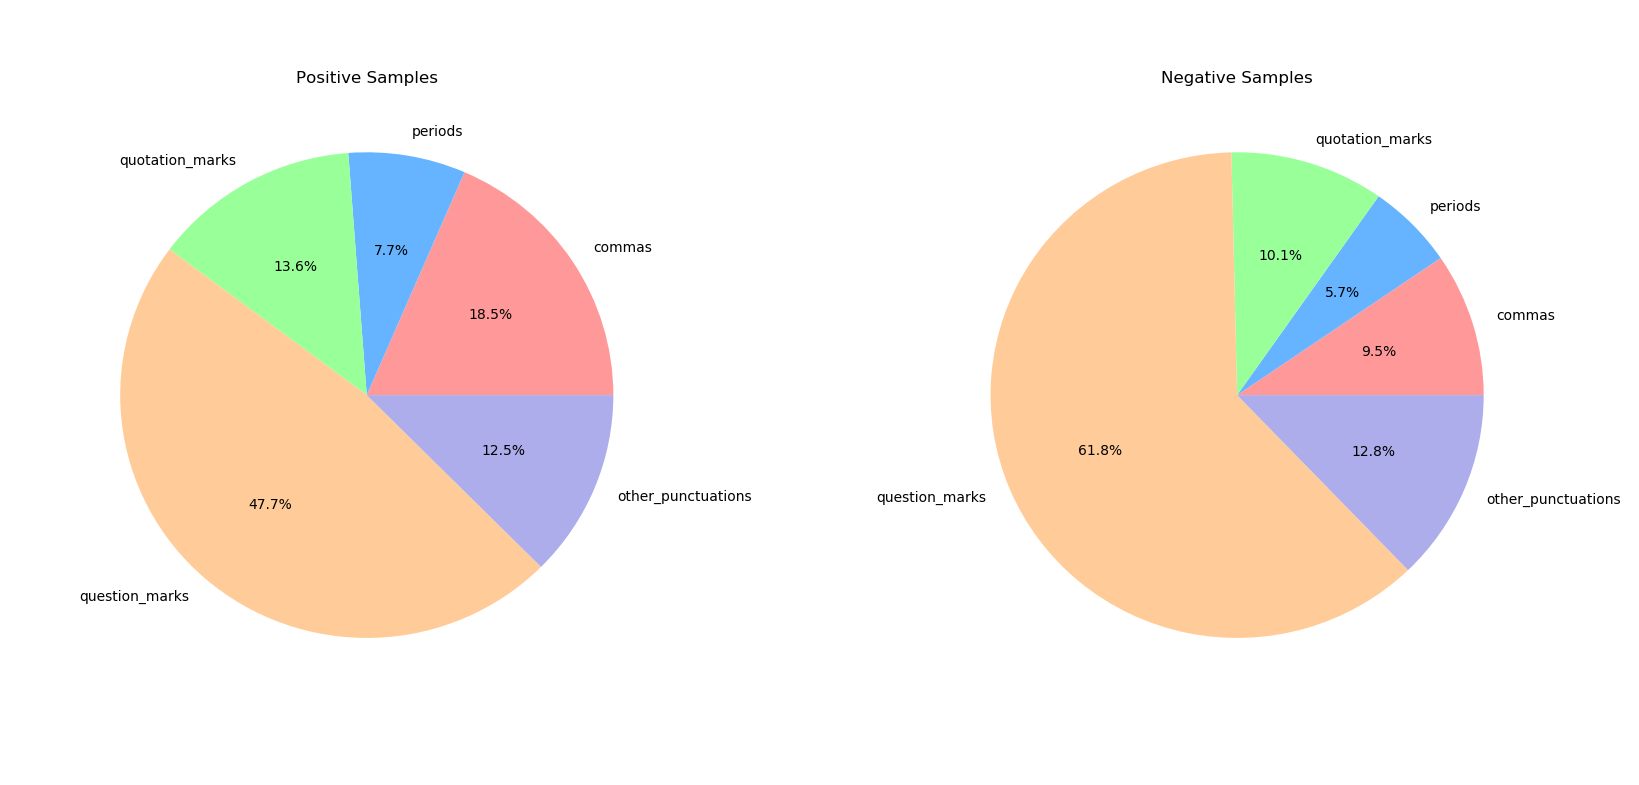
\includegraphics[width=\textwidth, center]{graphs/puncpiecharts.png}
	\caption{Pie charts for proportions of punctuations in positive and negative samples}
	\medskip
	\small
	\label{figure:puncpie}
\end{figure}

In addition to the statictical data, we also plan to visualize the word embeddings of labeled and unlabelled sentences. Consider the size of our corpus, we will first extract the most frequent unigrams, and visualize the correponding word vectors using appropriate methods such as t-SNE plots. 



\subsection{Experiments and Expectations}

Our experiments contain two primary goals: one is to investigate the performance of a similar architecture to state-of-art sarcasm detection models on insincerity classification; the other is to explore how pre-extracted corpus-statistical and sentiment features contribute to the classification results. 

Based on the similarities of the linguistic natures of sarcasm and rhetorical questions, we expect that our baseline CNN-LSTM model will achieve good performance on the task because similar models are proven to be successful in sarcasm detection. Once we achieve reasonable results with our baseline model, we will proceed to add different components of the pre-extracted data into the neural network and evaluate their effects on the results. Since information such as sentiment scores directly correlates with the indicators of insincere questions, we anticipate that directly feeding such information to the network, instead of relying on word embeddings as semantic representation, should improve our model's performance. Without empirical results, it is difficult to predict whether statistical features such as punctuation marks counts will augment our model. But consider that the distributions of extractednstatistical features were significantly different in labelled and unlabeled data population, we expect some improvements in the evaluation metrics.

Additionally, to understand the nature of insincere questions, we will use the statistical tests and visualization methods described in the previous sections to conduct analysis. We will compare and contrast the two populations to identify what aspects of the text tend to indicate insincerity. 


\section{Methodology}
\subsection{Problem Definition}

Let the dataset be $X = \left \{ X_1, X_2,\cdots, X_N \right \}$ so that $X_i = \left \{ t_1, t_2,\cdots, t_k \right \}$, where $t_i$ is the $i^{th}$ token, $i\in [1,k]$. Besides, we also have $Y={Y_1, Y_2,\cdots,Y_N}$ where $Y_i\in\left\{ 0, 1 \right\}$ so that 1 indicates the sample is labeled as  insincere. Firstly each textual sample would be embedded using both ELMo and corpus statistics (shown as model S) as:
\begin{align} 
\begin{split}
   R_i &= [ELMo1, ELMo2,\cdots,ELMo_k]\\
   C_i &= S(X_i)
\end{split}         
\end{align}
For model M taking $X_i$ as input, it would compute the output as $\widetilde{Y_i} = M(X_i) = M(R_i, C_i), \widetilde{Y_i} \in \left\{ 0, 1 \right\}$. Therefore, the performance of our model would be evaluated by:

\begin{align} 
\begin{split}
   Precision(X_i) &= Pr(Y_i=1 \mid \widetilde{Y_i}=1) \\
   Recall(X_i) &= Pr(\widetilde{Y_i}=1 \mid Y_i=1) \\ 
   F1 & = 2 * \frac{Precision(X_i) Recall(X_i)}{Precision(X_i) + Recall(X_i)}
\end{split}         
\end{align}
The aim of this project is to use corpus statistics to augment the performance of standard CNN-LSTM for insincerity classification.


\subsection{Word Embedding}

To better exploit information embedded in the short contexts of Quora questions, we applied Embeddings from Language Models(ELMo) to embed our text data into vector space for the downstream analysis instead of naive one-hot encoding.

A critical obstacle of language modeling is caused by the curse of dimensionality. To address this problem, in 2003, \citet{bengio2003neural} proposed a feed-forward Neural Network Language Model (NNLM) to learn a densely distributed representation\citep{hinton1986learning} for words, where both the word feature vectors and the parameters of that probability function were learned at the same time. NNLM is designed to learn $f \left( w _ { t } , \cdots , w _ { t - n + 1 } \right) = \hat { P } \left( w _ { t } | w _ { 1 } ^ { t - 1 } \right)$, $w _ { t } \in V$, where $w_1 \cdots w_T$ is the word sequence and $V$ is a large but finite vocabulary. This objective is divided into two steps: firstly, the previous N words would be mapped into real vectors by a share projection matrix, which represents each word of the vocabulary with a distributed feature vectors; then, the sequence of word feature vectors would be mapped into a probability distribution over $V$. As a result, this model yielded better perplexity compared to N-gram models and inspired more researchers to look into distributed representations of words.

Recognizing the need to include distributed representations of words introduced by \citet{hinton1984distributed}, \citet{mikolov2013efficient} analyzed NNLM and proposed two models to learn the words' continuous vector representations. Originally, NNLM mainly consisted of three layers: words were first mapped into embeddings at projection layer; then embedded vectors flowed into an ordinary hyperbolic tangent hidden layer; finally, the output layer represented the probability distribution over $V$. Therefore, most of the computation happened in the output layer. To learn the continuous word representations with higher accuracy and lower computational cost from a huge corpus, the first model Mikolov et al. proposed was the Continuous Bag-of-Words Model (CBOW) which removed the non-linear hidden layer. In CBOW, embedded words would be first projected and then averaged into the same position, after which an output layer would be presented with hierarchical softmax. They also provided another model that was similar to CBOW called Continuous Skip-gram Model to predict the context given a word. The result turned out to be promising as the model did not only extract the syntactic regularities but also revealed subtle semantic information of words.

% \textbf{Global Vectors for Word Representations(GloVe).} Although methods for word embeddings claimed great success in capturing syntactic and semantic properties, \citet{pennington2014glove} found that there were still drawbacks in the two major models: global matrix factorization and local context window methods. For instance, global matrix factorization performs poorly in word analogy task, while local context window methods like skip-gram fail to exploit the statistical information provided by copus. Therefore, they proposed a log-bilinear regression model that combines the advantages of the two models called Global Vectors for Word Representations, as the global corpus information are properly captured in this model. In designing their model, they first constructed a word-word co-occurance matrix $X$, where $X_{ij}$ refers to the number of times word $j$ appears in the context of word $i$. Then they defined $X_i=\sum_kX_{ik}$ indicating the number of times word $i$ serves as the context for any other word $k$. Finally, they let $P_{ij}=P(j|i)=X_{ij}/X_i$ be the probability of word $j$ appeared in the context of word $i$. With the ratios of co-occurance probabilities, they found that certain aspects of meaning could be well captured, therefore they encoded it into GloVe and achieved higher accuracy with lower computational cost.


As many previous models tried to embed words into same vectors, they failed to model polysemy properly. \citet{peters2018deep} therefore proposed the Embeddings from Language Models (ELMo) representations which is a new contextualized word representations to explore syntactic and semantic features of words and also how they vary in different contexts by embedding each token as a function of the input space. Normally, a language model would try to predict the next token given the previous context: $p \left( t _ { 1 } , t _ { 2 } , \ldots , t _ { N } \right) = \prod _ { k = 1 } ^ { N } p \left( t _ { k } | t _ { 1 } , t _ { 2 } , \ldots , t _ { k - 1 } \right)$. Instead, a backward language model processes the sentence reversly, trying to predict the previous token provided with the furture context: $p \left( t _ { 1 } , t _ { 2 } , \ldots , t _ { N } \right) = \prod _ { k = 1 } ^ { N } p \left( t _ { k } | t _ { k + 1 } , t _ { k + 2 } , \ldots , t _ { N } \right)$. ELMo adopted a bidirectional language model(biLM) which combines both forward and backward language models: $\sum _ { k = 1 } ^ { N } ( \log p \left( t _ { k } | t _ { 1 } , \ldots , t _ { k - 1 } ; \Theta _ { x } , \overrightarrow { \Theta } _ { L S T M } , \Theta _ { s } \right) + \log p \left( t _ { k } | t _ { k + 1 } , \ldots , t _ { N } ; \Theta _ { x } , \overleftarrow{\Theta } _ { L S T M } , \Theta _ { s } \right) )$. Therefore, for a \textit{L}-layer biLM using LSTM, there will be $2L+1$ representations for each token $t_k$:
\begin{align} 
\begin{split}
  R _ { k } & = \left\{ \mathbf { x } _ { k } ^ { L M } , \overrightarrow { \mathbf { h } } _ { k , j } ^ { L M } , \overleftarrow { \mathbf { h } } _ { k , j } ^ { L M } | j = 1 , \ldots , L \right\} \\ & = \left\{ \mathbf { h } _ { k , j } ^ { L M } | j = 0 , \ldots , L \right\},
\end{split}         
\end{align}
where $\mathbf { h } _ { k , 0 } ^ { L M }$ is token layer while ${ \mathbf { h } } _ { k , j } ^ { L M } = [\overrightarrow { \mathbf { h } } _ { k , j } ^ { L M } ; \overleftarrow { \mathbf { h } } _ { k , j } ^ { L M }]$ refers to biLSTM layers. Then, ELMo would integrate all representations into one single vector for each specific downstream NLP tasks with $\mathbf { E } \mathbf { L } \mathbf { M } \mathbf { o } _ { k } ^ { \operatorname { task } } = E \left( R _ { k } ; \Theta ^ { t a s k } \right) = \gamma ^ { \operatorname { task } } \sum _ { j = 0 } ^ { L } s _ { j } ^ { t a s k } \mathbf { h } _ { k , j } ^ { L M }$.

In our project, ELMo was applied and the task specific weighting of all three layers of representations shown as the equations 1 in  \citet{peters2018deep} (\textit{i.e.} character-convnet output and two LSTM outputs) would be find-tuned.


\subsection{Neural Networks}
\begin{figure}[ht!]
	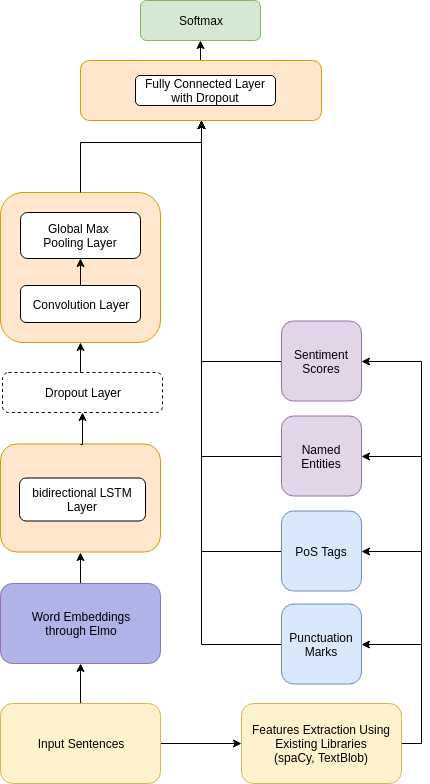
\includegraphics[height=0.7\textheight, center]{graphs/nn_architecture.png}
	\caption{Illustration of neural networks architecture}
	\medskip
	\small
	In this figure, the same types of components are shown in the same colours. The blocks with dashed lines correspond to layers that typically appear in a neural networks, but possibly hinder performance according previous studies. We decide to construct a baseline model without these layers, and add them in later to compare the performance if time allows. 
	\label{figure:nnarchitecture}
\end{figure}
Based on our review of neural nerworks models in the field of sentiment analysis, we decided to adopt a CNN-LSTM-DNN model as illustrated in Figure \ref{figure:nnarchitecture}. 

Studies have shown that compared to completely distributing word representations, modularized components with specific tasks could improve the overall performance of a CNN model \citep{poria2017}. As we discussed in the previous sections, we have established several characteristics that indicate a Quora question to be insincere; therefore, the idea of combining various components each responsible for detecting different classification clues can be valuable for our project. In our design, the network is generally divided into two components: a baseline CNN-LSTM model taking word vectors as inputs, and extracted syntactic and semantic features from existing libraries. Ideally, we will train the baseline model first, and feed the additional features (punctuation marks, named entities, PoS tags, and sentiment scores) one at a time to explore their effects on model performance. 

Among RNN implementations, LSTMs are advantageous because such architecture is easier to train and suffers less from vanishing or exploding gradients. The combination of CNN and RNN networks is also beneficial for the several reasons. First, convolutional layers help to extract abstract and compact features to be used as inputs to LSTM network \citep{chan2015}, which in turn compensates for the disadvantage of fixed filter width of convolutional layers, allowing for better analysis of long-distance relationships over texts with various length. Additionally, the convolution layers reduce feature variations so that CNN-LSTM work more efficiently \citep{ghosh2016}.

To combine different components, we plan to feed the output of LSTM layers and the pre-extracted features into a fully connected layer to match the features into a more separable space. Another design is to first feed the extracted features into a fully connected layer, and than concatenate the output of this layer with the output of LSTMs as the input vector for the final fully connected layer. We will then use softmax for classification and compute cross entropy as the loss function. 



\subsection{Evaluating Metrics}

In the \num[group-separator={,}]{1044839} training samples, there are \num[group-separator={,}]{980167} samples labeled as sincere while \num[group-separator={,}]{64672} of them are labeled as insincere. Therefore, $accuracy = \frac{ the\ number\ of\ correctly-classified\ samples}{the\ number\ of\ all\ samples}$ is not appropriate for evaluating the model. In this section, targeting at this biased dataset, different evaluation metrics will be discussed and applied.

There are two distinct values of \textit{target} in our dataset: 0 indicates a sincere question while 1 indicates a insincere one. In this project we define samples that are labeled as 1 to be positive while those labeled as 0 to be negative. Hence we could calculate model's precision, recall and F1 score accordingly. Provided that, these statistical metrics could be applied for evaluations.



%------------------------------------------------

%----------------------------------------------------------------------------------------
%	BIBLIOGRAPHY
%----------------------------------------------------------------------------------------
\newpage
\bibliographystyle{unsrt}

\bibliography{csc2511.bib}

%----------------------------------------------------------------------------------------

\end{document}